\section{Performance Evaluation}
\label{sec:results}

\begin{figure*}[ht]
  \centering
  \begin{minipage}{.33\textwidth}
    \centering
    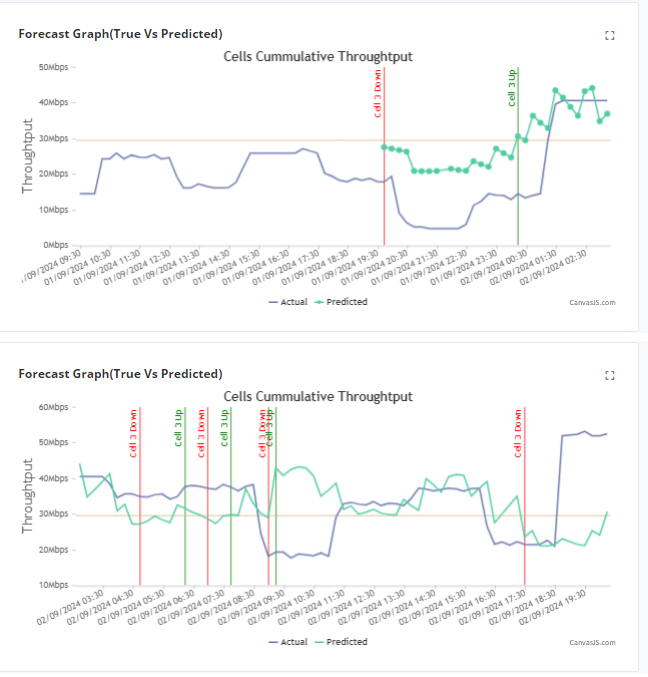
\includegraphics[width=\linewidth]{/Users/pulakmehrotra/Desktop/SaankhyaLabs/es_oran_paper/acm_version_final/images/results1.png}
    \caption{Functioning of our ES rApp over the NS-3 Simulator}
    \label{fig:r1}
  \end{minipage} % Add space here
  \begin{minipage}{.33\textwidth}
    \centering
    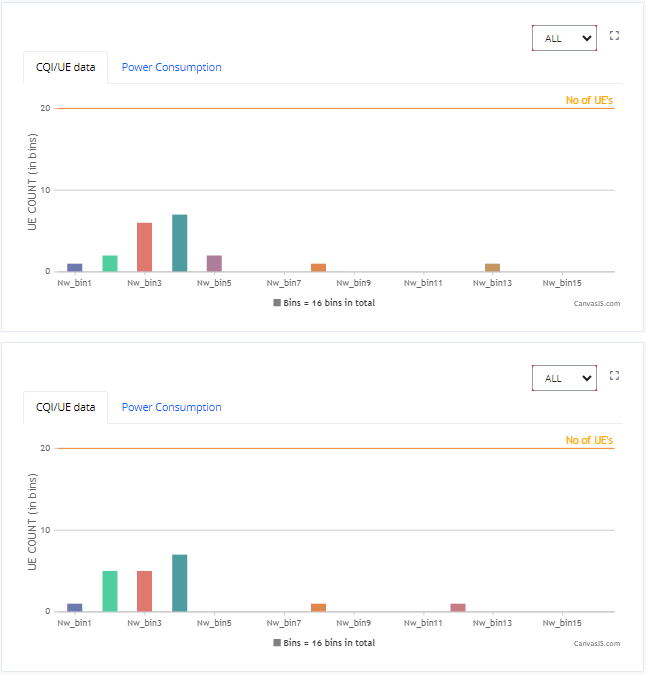
\includegraphics[width=\linewidth]{/Users/pulakmehrotra/Desktop/SaankhyaLabs/es_oran_paper/acm_version_final/images/results2.png}
    \caption{Comparison of CQI distributions before and after the implementation of cell shutdown}
    \label{fig:r2}
  \end{minipage}% % Add space here
  \begin{minipage}{.33\textwidth}
    \centering
    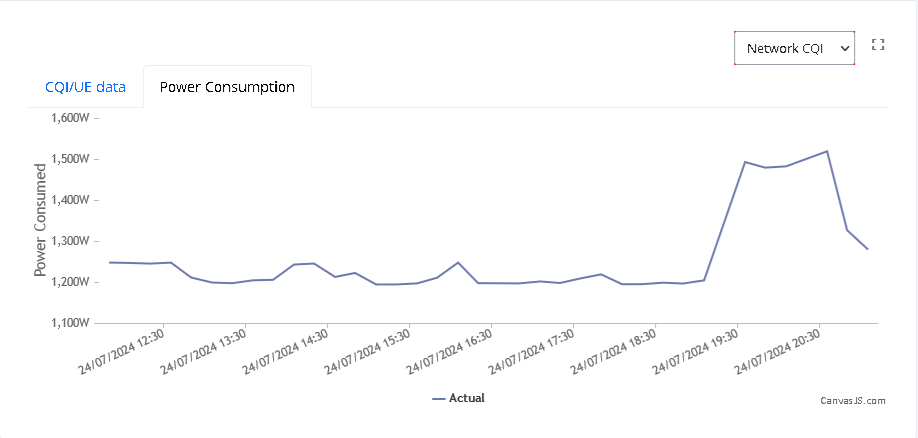
\includegraphics[width=\linewidth]{/Users/pulakmehrotra/Desktop/SaankhyaLabs/es_oran_paper/acm_version_final/images/results3.png}
    \caption{Power Consumption of the Setup over time}
    \label{fig:r3}
  \end{minipage}
\end{figure*}

In this section, we evaluate the performance of our proposed Energy Saving solution in our software-defined O-RAN network. 
%Our setup is lightweight, focusing primarily on evaluating the effectiveness of our proposed algorithm rather than the performance of the underlying simulations.
We first discuss the simulation setup, followed by the results of our experiment and a discussion on maintaining QoS guarantees.
In the ensuing graphs, to illustrate the long-term impact of the energy-saving algorithm, we've adopted a time conversion convention where 10 seconds equate to 15 minutes. 

\subsection{Simulation Setup}
Our solution is deployed as an independent rApp, interfacing with the Non-RT RIC and the A1 interface of the O-RAN stack. 
This rApp dispatches decision-making policies to the Near-RT RIC, which houses the TS xApp responsible for reallocating UEs during cell shutdown or bringup processes.
The network, simulated as a Digital Twin using an NS-3 Simulator \cite{ns3}, comprises eight cells with 20 User Equipments (UEs) per cell, operating in a single-threaded mode.
The rApp operates in a feedback loop with the Digital Twin, obtaining power readings, throughput, and other network characteristics across the coverage area.
The network is configured to operate in a 5G New Radio (NR) based CBRS network deployment.

\textit{Two Digital Twins?} The Digital Twin in use here is a different one as the one mentioned earlier in the paper.
For simplicity, we refer to the Digital Twin implemented with NS-3 as the 'NS-3 Simulator', and the one implemented with CloudRF as the 'Digital Twin'.
The Digital Twin integrated into the ES rApp, is a streamlined simulator that reports selected characteristics of the deployed system, implemented using CloudRF.
The NS-3 simulator serves as the backbone for our network simulation, encompassing the core network, the gNBs, and the UEs. 

\subsection{Power Consumption Reduction}

%The proposed algorithm ensures that the QoS guarantees are maintained during the cell shutdown and bringup processes.
%We try to ensure the policy proposed does not lead to a significant drop in the overall CQI of the channels in use for transmission.
We have conducted a series of experiments to evaluate the performance of our proposed solution especially focusing on the reduction in the power consumption over the given time-frame.
We look at the performance figures on how the forecasts of the overall throughput forecast helps achieve cell shutdown and bringup.
\hyperref[fig:r1]{Figure 3} depicts two scenarios of cell shutdown and activation: the upper scenario illustrates this process in a single-cell setup, while the lower scenario demonstrates it in an eight-cell configuration.
The LSTM-based Traffic Predictor effectively identifies the optimal times for shutdown and activation, as clearly demonstrated in the single-cell setup. 
Furthermore, our system has the capability to operate across multiple cells simultaneously.

The most straightforward method to observe a decrease in energy consumption involves continuously tracking the total power usage of the network, specifically within the NS-3 simulator.
In our implementation, we've incorporated monitoring hooks to track this value. 
The observed data is visualized in \hyperref[fig:r3]{Figure 5}.
In our simulations, we observed a 32\% reduction in power across short sample durations. 
We anticipate that the power savings could be significantly higher in longer and more complex setups.

\subsection{Maintaining QoS Guarantees}

In this section, we demonstrate how our setup maintains the QoS guarantees during system operation.
By utilizing the CQI data collected from all connected UEs, we can illustrate the system's CQI distribution at any given moment.
\hyperref[fig:r2]{Figure 4} illustrates the CQI distribution of the system before (depicted in the upper graph) and after (shown in the lower graph) the implementation of a cell shutdown policy.
The system's probability distribution experiences only minor changes, with a single CQI bin undergoing significant alterations.
This further substantiates that our ES solution preserves the channel quality for all UEs connected to the active eNBs, thereby ensuring the QoS.